\section{Formulation} \label{sec:formul}
The phase-field model as a diffuse interface model does not introduce discontinuities into the solid but the fracture surface is approximated by a scalar valued field. Thus, the boundary between damaged and not damaged areas is smoothed. In the following parts, a model for brittle and ductile fracture as well as a second- and fourth-order model are presented. At first, the notation and formulation considering brittle fracture is outlined. Afterwards, differences in the formulation considering ductile fracture are shown. For the rest of this paper, following notation is made (see \figref{fig:bodies}\subrefnew{fig:body_1}). The arbitraray body $\Omega\subset\mathbb{R}^{d}$ ($d\in\{1,2,3\}$) has external boundary $\partial\Omega$ and evolving internal discontinuity boundary (fracture surface) $\Gamma$. The displacement field at a given point $\mathbf{x}$ and time $t$ is given by $\mathbf{u}\left(\mathbf{x},t\right)\in\mathbb{R}^{d}$. Dirichlet boundary conditions $\mathbf{u}\left(\mathbf{x},t\right)=\mathbf{g}\left(\mathbf{x},t\right)$ on $\partial\Omega_{\mathbf{g}}$ and Neumann boundary conditions $\mathbf{t}\left(\mathbf{x},t\right)=\mathbf{h}\left(\mathbf{x},t\right)$ on $\partial\Omega_{\mathbf{h}}$ are imposed with $\partial\Omega_{\mathbf{g}}\cup\partial\Omega_{\mathbf{h}}=\partial\Omega$. $\mathbf{t}\left(\mathbf{x},t\right)$ describes a given traction vector force.
\begin{figure}[ht!]
    \centering
    \begin{subfigure}[t]{0.4\textwidth}
        \centering
        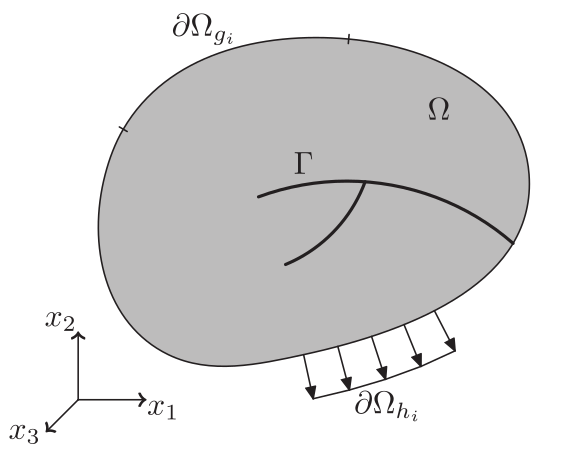
\includegraphics[scale=0.3]{data/Body_1}
        \caption{}\label{fig:body_1}
    \end{subfigure}
    %
    \begin{subfigure}[t]{0.5\textwidth}
        \centering
        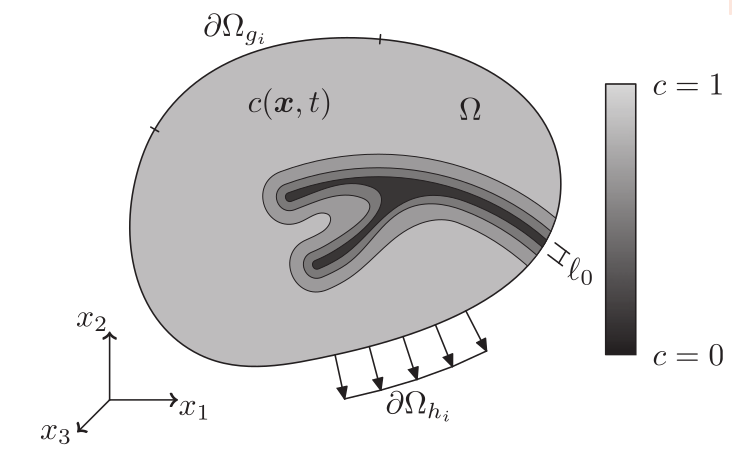
\includegraphics[scale=0.3]{data/Body_2}
        \caption{}\label{fig:body_2}
    \end{subfigure}
    \caption{\subrefnew{fig:body_1} Representation of a solid body $\Omega$ and internal discontinuitiy boundary $\Gamma$. \subrefnew{fig:body_2} Phase-field approximation of $\Gamma$. $c\left(\mathbf{x},t\right)$ describes the phase-field and $l_{0}$ is a parameter for controlling the failure zone's width. \cite{01_PF_dyn_brittle}} \label{fig:bodies}
\end{figure}


\subsection{Griffith's theory of brittle fracture} \label{sec:formul_Griffith}
Considering small derformations and deformation gradients, the small strain tensor $\mathbf{\epsilon}\left(\mathbf{x},t\right)$ is given by
\begin{equation}
	\bm{\varepsilon} = \nabla^{s}\mathbf{u}
\end{equation}
where $\cdot^{s}$ refers to the symmetric part. Considering isotropic linear elasticity, the undamaged elastic energy densitiy can be expressed by
\begin{equation} \label{eq:psi_e}
	\Psi_ {e}\left(\bm{\varepsilon}\right) = \dfrac{1}{2}\lambda tr\left(\bm{\varepsilon}\right)^{2}+\mu\bm{\varepsilon}:\bm{\varepsilon}
\end{equation}
using the Lam\'{e} constants $\lambda$ and $\mu$.

According to the energetic approaches to fracture, the critical fracture energy density $\mathcal{G}_{c}$ defines the energy being necessary to create a unit area of fracture surface. Since translation of cracks shall be forbidden and extension, branching and merging shall be allowed, there is an irreversibility condition stating $\Gamma\left(t\right)\subseteq\Gamma\left(t+\Delta t\right), \forall \Delta t>0$.

However, Griffith's fracture theory reaches its limits as soon as it is used to predict crack paths, nucleation of new cracks, complicated crack behaviours during kinking and branching. Thus, the problem is formulated in a variational sense which is shown in the following paragraphs. The phase-field approach can then be seen as a regularized version of this variational formulation. \citep{05_PF_ductile}

Newton's laws follow Hamilton's principle stating that the functional 
\begin{equation}
	J\left(q,\dot{q}\right)=\int\limits_{t_{0}}^{t_{1}}\mathcal{L}\left(q,\dot{q},t\right)\mathrm{d}t
\end{equation} reaches a stationary point. $\mathcal{L}\left(q,\dot{q},t\right)$ describes the so called Lagrangian and $q$ represents generalized coordinates. The motion of the mechanical system from $t_{0}$ to $t_{1}$ is then captured by this formulation \citep{01_B_LagrMech}. In our case, the Lagrangian reads $\mathcal{L}\left(\mathbf{u},\dot{\mathbf{u}},\Gamma\right)=\Psi_{kin}\left(\mathbf{u}\right)-\Psi_{pot}\left(\mathbf{u},\Gamma\right)$. Inserting the introduced cricical fracture energy densitiy $\mathcal{G}_{c}$, the kinetic energy of the body and \eqref{eq:psi_e} leads to
\begin{equation} \label{eq:lagr}
	\mathcal{L}\left(\mathbf{u},\dot{\mathbf{u}},\Gamma\right) = \int\limits_{\Omega}\left(\frac{1}{2}\rho\dot{\mathbf{u}}\dot{\mathbf{u}}-\Psi_{e}\left(\bm{\varepsilon}\right)\right)\mathrm{d}\Omega - \int\limits_{\Gamma}\mathcal{G}_{c}\mathrm{d}\Gamma.
\end{equation}
The Euler-Lagrange Equation (ELE) is a differential equation which solution satisfies equilibrium. Thus, this equation is also called the equation of motion \footnote{The term \textit{equation of motion} may be a bit misleading. It refers to the differential equation and not to its solution.}. A minimizer $q$ for \eqref{eq:lagr} satisfies the ELE
\begin{equation} \label{eq:ELE_O2}
	\dfrac{\partial\mathcal{L}}{\partial q}-\dfrac{\mathrm{d}}{\mathrm{d}t}\dfrac{\partial\mathcal{L}}{\partial\dot{q}}=0.
\end{equation}
For a given $\mathcal{L}=\mathcal{L}\left(q,\dot{q},\ddot{q}, t\right)$ this differential equation is changed to
\begin{equation} \label{eq:ELE:_O4}
	\dfrac{\partial\mathcal{L}}{\partial q}-\dfrac{\mathrm{d}}{\mathrm{d}t}\dfrac{\partial\mathcal{L}}{\partial\dot{q}}+\dfrac{\mathrm{d}^{2}}{\mathrm{d}t^{2}}\dfrac{\partial\mathcal{L}}{\partial\ddot{q}}=0
\end{equation}
\citep{01_B_LagrMech}. So as to circumvent problems of algorithmically tracking the propagating dicontinuity $\Gamma$, the phase-field approach will be presented in the next chapters which regularizes the just mentioned variational formulation.

\subsection{Phase-field approximation} \label{sec:ph_approx}
As can be seen in \figref{fig:bodies}\subrefnew{fig:body_2} the fracture surface $\Gamma$ is approximated by a scalar valued field $c\left(\mathbf{x},t\right)$. This field is called the phase-field. Values of $c=1$ represent regions away from the crack (undamaged material) whereas $c=0$ symbolizes the crack. Now, in \eqref{eq:lagr} the surface integral and thus, the need for tracking the crack can be eliminated.
